%!TEX root = optimization1718.tex

\chapter{Non-Euclidean setting: Frank-Wolfe}
\emph{Speaker: Chris Carmona, 23/10/2017.}\\

The \emph{Conditional Gradient Descent} method, also known as \emph{Frank-Wolfe} is an iterative first-order optimization algorithm for constrained convex optimization, originally proposed in \cite{Frank1956} by Marguerite Frank and Philip Wolfe, then post-docs working in the Princeton logistics project led by Kuhn and Tucker. In recent years, Frank-Wolfe-type methods have re-gained interest, started by the valuable insights provided by \cite{Jaggi2013}, and fuelled by its good scalability and convergence properties properties (eg. convergence invariance under affine transformations).

The method addresses general constrained convex optimization problems of the form $\min_{x \in \X} f(x)$. It assumes that the objective function $f$ is convex and continuously differentiable, and that the domain $\X$ is a compact convex subset of any vector space. Procedure \ref{alg:frank_wolfe} describes the method. In each iteration, the algorithm considers a linear approximation of the objective function, and moves towards a minimizer of this linear function, taken over the domain $\X$. Figure \ref{fig:frank_wolfe} illustrates one iteration of the algorithm (the domain $\X$ is denoted by $\mathcal{D}$ here).

\begin{algorithm}
%\scriptsize
\caption{Conditional Gradient Descent (Frank-Wolfe)}
   \begin{algorithmic}[1] \label{alg:frank_wolfe}
   \REQUIRE $f$ a differentiable and convex function on $\X$ that is $\beta$-smooth w.r.t. some norm $\|\cdot\|$.
   \ENSURE $x_T$ such that $f(x_T)-f(x^\ast) \leq \frac{4 \beta R^2 }{T+1}$ with $R = \sup_{x,y \in \X} \| x - y\|$
   
   \STATE Let $x_{0} \in \X$
   \FOR {$t \in 0,\ldots,T$}
      \STATE Set $\gamma_t=\frac{2}{t+2}$
      \STATE Compute
      \begin{equation} \label{eq:fw_update}
      s_t:= \argmin_{s \in \X } \langle s, \nabla f(x_t) \rangle
      \end{equation}
      \STATE Update $x_{t+1} := (1-\gamma_t)x_t+ \gamma_t s_t = x_{t} + \gamma_t (s_t-x_t)$
   \ENDFOR
   \STATE {\bfseries return} $x_T$
\end{algorithmic}
\end{algorithm}

From a computational perspective, a key property of this scheme is that it replaces the projection step of projected gradient descent by a linear optimization over $\X$ , which in some cases can be a
much simpler problem.

\begin{figure}[ht]
\begin{center}
   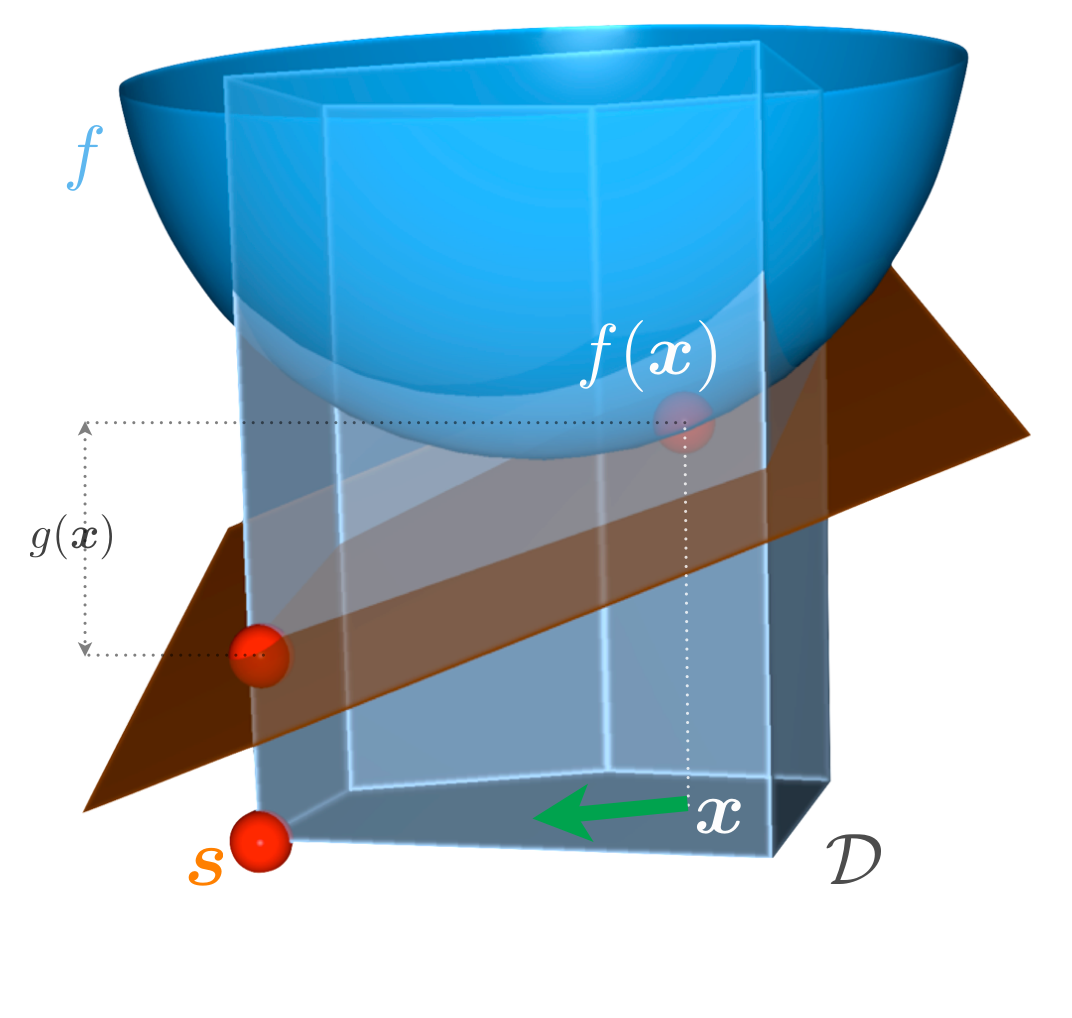
\includegraphics[width=0.5\textwidth]{img/frank_wolfe}
\end{center}
   \caption{Graphical representation of the Conditional Gradient Descent algorithm \cite{Jaggi2013}}
   \label{fig:frank_wolfe}
\end{figure}


\section{Convergence analysis.}

A major advantage of conditional gradient descent over projected gradient descent is that the former can adapt to smoothness in an arbitrary norm.

\if
The convergence analysis of Frank-Wolfe type algorithms crucially relies on a measure of “non-linearity” of our objective function f over the domain $\X$. The \emph{curvature constant} $C_f$ of a convex and differentiable function $f:\mathbb{R}^n \rightarrow \mathbb{R}$, with respect to a compact domain $\X$ is defined as:

\begin{equation} \label{eq:curv_const}
C_f := \sup_{ \substack{x,s \in \X,\\ \gamma \in [0,1],\\ y=x+\gamma(s-x)} } \frac{2}{\gamma^2} (f(y)-f(x)-\nabla f(x)^\top (y-x))
\end{equation}

Note that $C_f$ actually measures how far $f$ is from being linear, getting $C_f=0$ when $f$ is linear. The quantity $f(y)-f(x)-\nabla f(x)^\top (y-x)$ is called the \emph{Bregman divergence} defined by $f$.
\fi

The following theorem establishes a bound of convergence. Note that the number of iterations needed to have $f(x_t)-f(x^*) \leq \epsilon$  is $O(\frac{1}{\epsilon})$.

\begin{theorem}
Let f be a convex and $\beta$-smooth function w.r.t. some norm $\|\cdot\|$, $R=\sup_{x,y \in \X} \| x-y \|$, and $\gamma_t=\frac{2}{t+1}$ for $t \geq 1$. Then for any $t\geq2$, one has:
\begin{equation}
f(x_t)-f(x^*) \leq \frac{4 \beta R^2 }{t+1}
\end{equation}
\end{theorem}

\begin{proof}
First, note that the following inequalities hold:
  \begin{align}
    f(x_{t+1})-f(x_t) & \leq \nabla f(x_t)^\top (x_{t+1}-x_{t}) + \frac{\beta}{2} \| x_{t+1}-x_{t} \|^2 \nonumber && \text{($f$ is $\beta$-smooth)} \\
    & \leq \gamma_t \nabla f(x_t)^\top (s_{t}-x_{t}) + \frac{\beta}{2} \gamma_t^2 R^2 \nonumber && \text{($x_{t+1}=x_t+\gamma (s_t-x_t)$)} \\
    & \leq \gamma_t \nabla f(x_t)^\top (x^*-x_t) + \frac{\beta}{2} \gamma_t^2 R^2 \nonumber && \text{(by definition $s_t \leq x^*$)} \\
    & \leq \gamma_t ( f(x^*)-f(x_t)) + \frac{\beta}{2} \gamma_t^2 R^2 \nonumber && \text{(convexity of $f$)}
  \end{align}
If we define $\delta_t = f(x_t)-f(x^*)$ then we get:
\begin{equation}
\delta_{t+1} \leq (1-\gamma_t)\delta_t+\frac{\beta}{2} \gamma_t^2 R^2
\end{equation}
Finally, the result is proved by induction using $\gamma_t =\frac{2}{t+1}$. We initialize at step 2, $t=1$, with the above inequality yielding $\delta_2 \leq \frac{\beta}{2} R^2$.
\end{proof}

\section{Sparse iterates property.}
In addition to being projection-free and "norm-free", the conditional gradient descent satisfies a perhaps even more important property: it produces \emph{sparse iterates}.

Consider the situation where $\X \subset \mathbb{R}^n$ is a polytope, that is the convex hull of a finite set of points (these points are called the vertices of $\X$ ). Then Caratheodory's theorem states that any point $x \in \X$ can be written as a convex combination of at most $n+1$ vertices of $\X$ . On the other hand, by definition of the conditional gradient descent, one knows that the $t$-th iterate $x_t$ can be written as a convex combination of $t$ vertices (assuming that $x_1$ is a vertex). Thanks to the dimension-free rate of convergence one is usually interested in the regime where $t<<n$, and thus we see that the iterates of conditional gradient descent are very sparse in their vertex representation.

\section{Application: Regularized least-squares regression.}
The three properties of conditional gradient descent (projection-free, norm-free, and sparse iterates) are critical to develop a computationally efficient procedure in solving this kind of problems.

Consider the regularized least-squares regression problem (which includes the LASSO). We would like to approximate a signal $Y \in \mathbb{R}^n$ by using a combination of few of the columns $x_j; j\in 1,\ldots,p$ in the matrix $X \in \mathbb{R}^{n \times p}$. Then, for a fixed $\lambda$ we have the penalized problem in dimension $p$:
\begin{equation}
\min_{\beta \in \mathbb{R}^p} \| Y - X \beta \|_2^2 + \lambda \|\beta\|_1 \nonumber
\end{equation}

Instead of considering the penalized version of the problem one could look at the following constrained problem, with $s \in \mathbb{R}$ fixed:
\begin{align} \label{eq:lasso_fw}
\min_{\beta \in \mathbb{R}^p} \| Y/s - X \beta \|_2^2 \\
\text{subject to} \|\beta\|_1 \leq 1 \nonumber
\end{align}

We are interested in situations where $n<<p$, that is the number of variables $p$ in $X$ can be very large, potentially exponential in the dimension $n$. Nonetheless we want to restrict our attention to algorithms that run in reasonable time with respect to $n$, that is we want polynomial time algorithms in $n$. Of course in general this is impossible, and we need to assume that the dictionary has some structure that can be exploited. Here we make the assumption that one can solve in time $p(n)$ (where $p$ is polynomial) the following problem for any $y\in\mathbb{R}^n$:
\begin{equation}
\min_{ 1\leq i \leq p } y^{\top} x_i\nonumber
\end{equation}
Finally, for normalization issues, we assume that the $\ell_2$-norm of the $x_i$'s are controlled by some $m > 0$, that is $\| x_j \|_2 \leq m, \forall j \in 1,\ldots,p $

Our problem of interest \ref{eq:lasso_fw} corresponds to minimizing the function $f(\beta) = \frac{1}{2}\| Y - X \beta \|_2^2 $ on the $\ell_1$-ball of $\mathbb{R}^p$ in polynomial time in $n$. At first sight this task may seem completely impossible indeed one is not even allowed to write down entirely a vector $\beta \in \mathbb{R}^b$ (since this would take time linear in $p$ ). The key property that will save us is that this function admits sparse minimizers as we discussed above, and this will be exploited by the conditional gradient descent method.

Let us study the computational complexity of the $t$-th step of
conditional gradient descent. First, observe that:
\begin{equation}
\nabla f (\beta)=X^\top (X\beta-Y) \nonumber
\end{equation}

Now assume that $z_t=X \beta_t - Y \in \mathbb{R}^n$ is already computed, then to compute the update \ref{eq:fw_update} one needs to find  the coordinate $i_t \in 1,\ldots,p$ that maximizes $| [\nabla f(\beta_t)](i) |$ which can be done by maximizing $x_i^\top z_t$ and $-x_i^\top z_t$. Thus the update \ref{eq:fw_update} takes time $O(p(n))$
\begin{equation}
x_{t+1} = (1+\gamma_t) x_t + \gamma_t \cdot sign( \nabla f(x_t)_{i_t} ) \cdot e_{i_{t}}
\end{equation}

Computing $\beta_{t+1}$ from $\beta_t$ and $i_t$ takes time $O(t)$ since $\|\beta_t \|_0 \leq t$, and computing $z_{t+1}$ from $z_t$ and $i_t$ takes time $O(n)$. Thus the overall time complexity of running t steps is (we assume $p(n) =\Omega(n)$)
\begin{equation} \label{eq:lasso_time_bound}
O(tp(n) + t^2 )
\end{equation}

To derive a rate of convergence it remains to study the smoothness
of $f$ . This can be done as follows:
\begin{align}
\| \nabla f(\beta) - \nabla f(\gamma) \|_{\infty} & = \| X^\top X(\beta-\gamma) \|_{\infty} \nonumber \\
& = \max_{1 \leq j \leq p} | x_j^\top \sum_{k=1}^{p} x_k(\beta(k)-\gamma(k)) | \nonumber \\
& \leq m^2 \| \beta-\gamma \|_1 \nonumber \\
\end{align}
which means that $f$ is $m^2$-smooth with respect to the $\ell_1$-norm.

Thus we get the following rate of convergence:
\begin{equation} \label{eq:lasso_fw_bound}
f(\beta_t)-f(\beta^*) \leq \frac{8 m^2}{t+1}
\end{equation}

Putting together \ref{eq:lasso_time_bound} and \ref{eq:lasso_fw_bound} we proved that one can get an $\epsilon$-optimal solution to \ref{eq:lasso_fw} with a computational effort of $O(m^2 p(n)/\epsilon+m^4/\epsilon^2)$ using the conditional gradient descent.

\section{Frank-Wolfe variants.}

\subsubsection{Line search.}

Instead of using the pre-defined step-sizes $\gamma=\frac{2}{k+2}$ a modified algorithm the best point on the line segment between the current iterate x(k) and s.
\begin{equation}
\gamma_t = \argmin_{\gamma \in [0,1]} f( x_{t-1} + \gamma(s_{t-1}-x_{k-1}) ) \nonumber
\end{equation}

\subsubsection{Fully corrective.}

This is a harder-working variant of the Frank-Wolfe method, which after the addition of a new \emph{atom} (or search direction) $s$ re-optimizes the objective $f$ over all previously used atoms. The change consists on computing $x_{t+1}$ using a convex combination of all the previous atoms $s_t$. This is:
\begin{equation}
x_{t+1} = \argmin_{x \in \text{conv}(s_0,\ldots,s_{t}) } f(x)
\end{equation}
Comparing to the original Frank-Wolfe method, the idea is that the variant here will hopefully make more progress per iteration, and therefore result in iterates $x$ being combinations of even fewer atoms (i.e. better sparsity). This however comes at a price, namely that the internal problem in each iteration can now become as hard to solve as the original optimization problem, implying that no global run-time guarantees can be given for the algorithm in general.

\subsubsection{Away steps.}
Another important variant is the use of \emph{away-steps}. The idea is that in each iteration, we not only add a new atom $s$, but potentially also remove an old atom (provided it is bad with respect to our objective). This requires that the iterate $x$ is represented as a convex combination of the current atoms. This variant can improve the sparsity of the iterates. Using away-steps, a faster linear convergence can be obtained for some special problem class.

\subsubsection{Inexact updates.}
Jaggi (2011) also analyzes inexact Frank-Wolfe updates.

Suppose we choose $s_t$ with some "small" inaccuracy so that:
\begin{equation}
      \langle s_t, \nabla f(x_t) \rangle = \min_{s \in \X } \langle s, \nabla f(x_t) \rangle + \delta \frac{\gamma_{t+1}C_f}{2}
\end{equation}

where $\delta$ is our \emph{inaccuracy parameter}. $C_f$ is known as the \emph{curvature constant}, measures how far $f$ is from being linear, getting $C_f=0$ when $f$ is linear, and defined as:
\begin{equation} \label{eq:curv_const}
C_f := \sup_{ \substack{x,s \in \X,\\ \gamma \in [0,1],\\ y=x+\gamma(s-x)} } \frac{2}{\gamma^2} (f(y)-f(x)-\nabla f(x)^\top (y-x))
\end{equation}


In \cite{Jaggi2013} it is shown that the attained rate of convergence is basically the same under this \emph{inexact updates}.

\begin{theorem}
The Conditional Gradient Method using fixed step $\gamma_t=\frac{2}{t+2}$ sizes and inaccuracy parameter $\delta \geq 0$,
satisfies
\begin{equation}
f(x_t)-f(x^*) \leq \frac{2 C_f }{t+2} (1+\delta)
\end{equation}
\end{theorem}
